\chapter{Ionization}
\label{chap:ionization}

In this chapter the model presented before is modified by introducing a small oscillating  external voltage. This perturbation allows the Majorana state to excite into continuum --- the process we will call ionization. The main goal here is to find the ionization rate when the typical size of the photon is much smaller than the spectrum gap.  Only regime with $ \abs{g_L}\ll g_R $ is considered --- this significantly simplifies the calculation, but still exhibits non-trivial physics with a number of different subregimes. 

\section{Introducing the perturbation}

 The perturbation is introduced as an oscillating	 voltage applied to the junction. This alters the Hamiltonian (\ref{full_hamiltonian}) in two ways --- by the modification of the chemical potentials $ \mu_L, \mu_R $ and by making the superconducting phase difference $ \varphi=\phi_R-\phi_L $ time dependent. The second effect is governed by the Josephson relation:
\begin{gather}
	U\br{\tau}
	=
	\frac{\hbar}{2e}
	\frac{\partial\varphi\br{\tau}}{\partial \tau}
\end{gather}

The ionization voltage is assumed to be small compared to other energy parameters, and this smallness is present in both effects. However, if the frequency $ \omega $ of voltage is also small, the perturbation in $ \Delta $ induced by the second effect will have additional big multiplier $ \frac{\Delta}{\omega} $ and will dominate the perturbation in $ \mu $. In this chapter only this regime is considered.

Time dependence of phase difference is introduced as:
\begin{gather}
	\varphi\br{\tau}=\varphi_0+\alpha\cos\omega \tau
\end{gather}
where $ \varphi_0 $ is an initial time independent phase difference and $ \alpha\ll1 $ is the amplitude of phase oscillations.

As was shown in section  \ref{sec:elimintaing_long-wave}, there is a gauge transform $ U_\phi $, which  redistributes the phase difference between the wires, so the phase in a given wire can have any value. This ambiguity just reflects a  fact, that only phase difference $ \varphi $ is an observable quantity, but not the phases $ \phi_L $, $ \phi_R $ separately. However, when treating the time dependent  phase difference this gauge transform also becomes time-dependent. After its application the additional term $ \dot{U}_{\phi\br{\tau}}U_{\phi\br{\tau}}^\dagger \propto \dot{\phi}\br{\tau}$ will appear, but, as $ \omega $ is small, it can be neglected. The corresponding condition on $ \omega $ will be established in section \textbf{ENTER SECTION}  

As the term $ \dot{U}_{\phi\br{\tau}}U_{\phi\br{\tau}}^\dagger \propto \dot{\phi}\br{\tau}$ is negligible, we again can gauge all the phase difference into the boundary condition. Now the boundary condition is time-dependent. It's not very convenient, and to avoid dealing with it we reformulate the problem in terms  of tunnel Hamiltonian, which allow us to treat both tunneling and time dependence simultaneously via perturbation theory.


\if 0

We introduce the time-dependent phases as: $ \phi_L=-\frac{\varphi_0}{2}-\frac{\alpha}{2}\cos \omega t $, $ \phi_R=-\phi_L=\frac{\varphi_0}{2}+\frac{\alpha}{2}\cos \omega t $. Thus the superconducting terms in the wire Hamiltonians alter: $ \Delta_{\pm\frac{\varphi}{2}} \to\Delta_{\pm\frac{\varphi}{2}\pm \frac{\alpha}{2}\cos \omega t} $. Decomposing them in small $ \alpha $ one can explicitly write the perturbation and try to compute the ionization rate. However this way appears to be quite difficult as the overlaps of all the states 
present in both wires and at first it seems that the Majorana states has too much ways to ionize. To avoid this difficulty, the tunnel Hamiltonian approach is used.

\fi

\section{Tunnel Hamiltonian approach}
\label{sec:tunnel_hamiltonian}
The main idea of this method is to hide all the time dependence and the tunnel effect in one single operator. To do so we need to rewrite the Hamiltonian as $ H=H_L+H_R+H_T $, where $ H_{L,R} $ are the Hamiltonians of the left and right wire without any contact (corresponding to zero tunneling: $ t=0 $), and $H_T  $ is a tunnel Hamiltonian both containing the time dependence and mixing the wavefunctions from different wires. 
Here the following notation is used: the Hamiltonians $ H_L $, $ H_R $ and $ H_T $ are 8x8 matrices in combined Nambu-Gorkov and LR-space. In LR-space they have the following form:
\begin{gather}
\label{tunnel_Hamiltonian_formalizm}
	H_L
	=
	\begin{pmatrix}
	h_L & 0 \\
	0 & 0
	\end{pmatrix}_{LR}
	\quad
	H_R
=
\begin{pmatrix}
0 & 0 \\
0 & h_R
\end{pmatrix}_{LR}
\quad
	H_T
=
\begin{pmatrix}
0 & h_T \\
h_T^\dagger & 0
\end{pmatrix}_{LR}	
\end{gather}
The Hamiltonians $ h_L $ and $ h_R $ eventually coinside with (\ref{bulk_Hamiltonian}) with zero boundary condition. The Hamiltonian $ h_T $ in unknown -- the goal is to make it in a way the corrections for the wavefunctions are restored . This wavefunctions and their  first tunneling corrections are listed in  appendix \ref{app:wavefunctions_with_corrections}.

The derivation of tunnel Hamiltonian matrix elements is presented in appendix \ref{app:tunnel}. Using the notation  $ \big|\gamma_{0}\,\big> $ for Majorana state and $ \big|\varepsilon,L_{0}\,\big> $, $ \big|\varepsilon,R_{0}\,\big> $ for continuous spectra, we have the following:
\begin{gather}
H_T=
\left(e^{i\frac{\varphi}{2}}+e^{-i\frac{\varphi}{2}}\right)
\tilde{H}_{T}
=
\left(e^{i\frac{\varphi}{2}}+e^{-i\frac{\varphi}{2}}\right)
\begin{pmatrix}
0 & \tilde{h}_{T} \\
\tilde{h}_T^\dagger & 0
\end{pmatrix}
\\
\label{tunnel_matrix_elements_maj-cont}
	\big<\gamma_{0}\,\big|\tilde{h}_{T}^{\dagger}\big|E,L_{0}\,\big>
	=
	4\sqrt{ug_{R}}
	t\zeta^{2}
	f\br{\frac{E}{\abs{g_L}}}
	\\
	\label{tunnel_matrix_elements_cont-cont}
	\big<\epsilon,R_{0}\,\big|\tilde{h}_{T}^{\dagger}\big|E,L_{0}\,\big>
	=
	-16u\zeta^{2}t
	f\br{\frac{E}{\abs{g_L}}}
	f\br{\frac{\varepsilon}{g_R}}
\end{gather}
where $ f\br{x}=\sqrt{x^2-1}\br{x+\sqrt{x^2-1}} $. Note, that $ \tilde{h}_{T} =\tilde{h}_{T}^\dagger $.

 The fact, that all energy dependences here are described by a single function $ f\br{x} $ insinuates that maybe it's possible to make this calculations in a more beautiful way.

\section{Ionization rate for $ g_R\gg\abs{g_L} $}


\subsection{Time dependence of perturbation}

To obtain the ionization rate one should treat $ H_T $ as perturbation. For unperturbed system, described with $ H_0=H_R+H_L $, the electrons cannot get from wire to another, but $ H_T $ allows these processes, so the ionization can be described as a set of jumps from right to left wire (see fig. \ref{fig:tunneling}).

\begin{figure}[H]
	\centering
	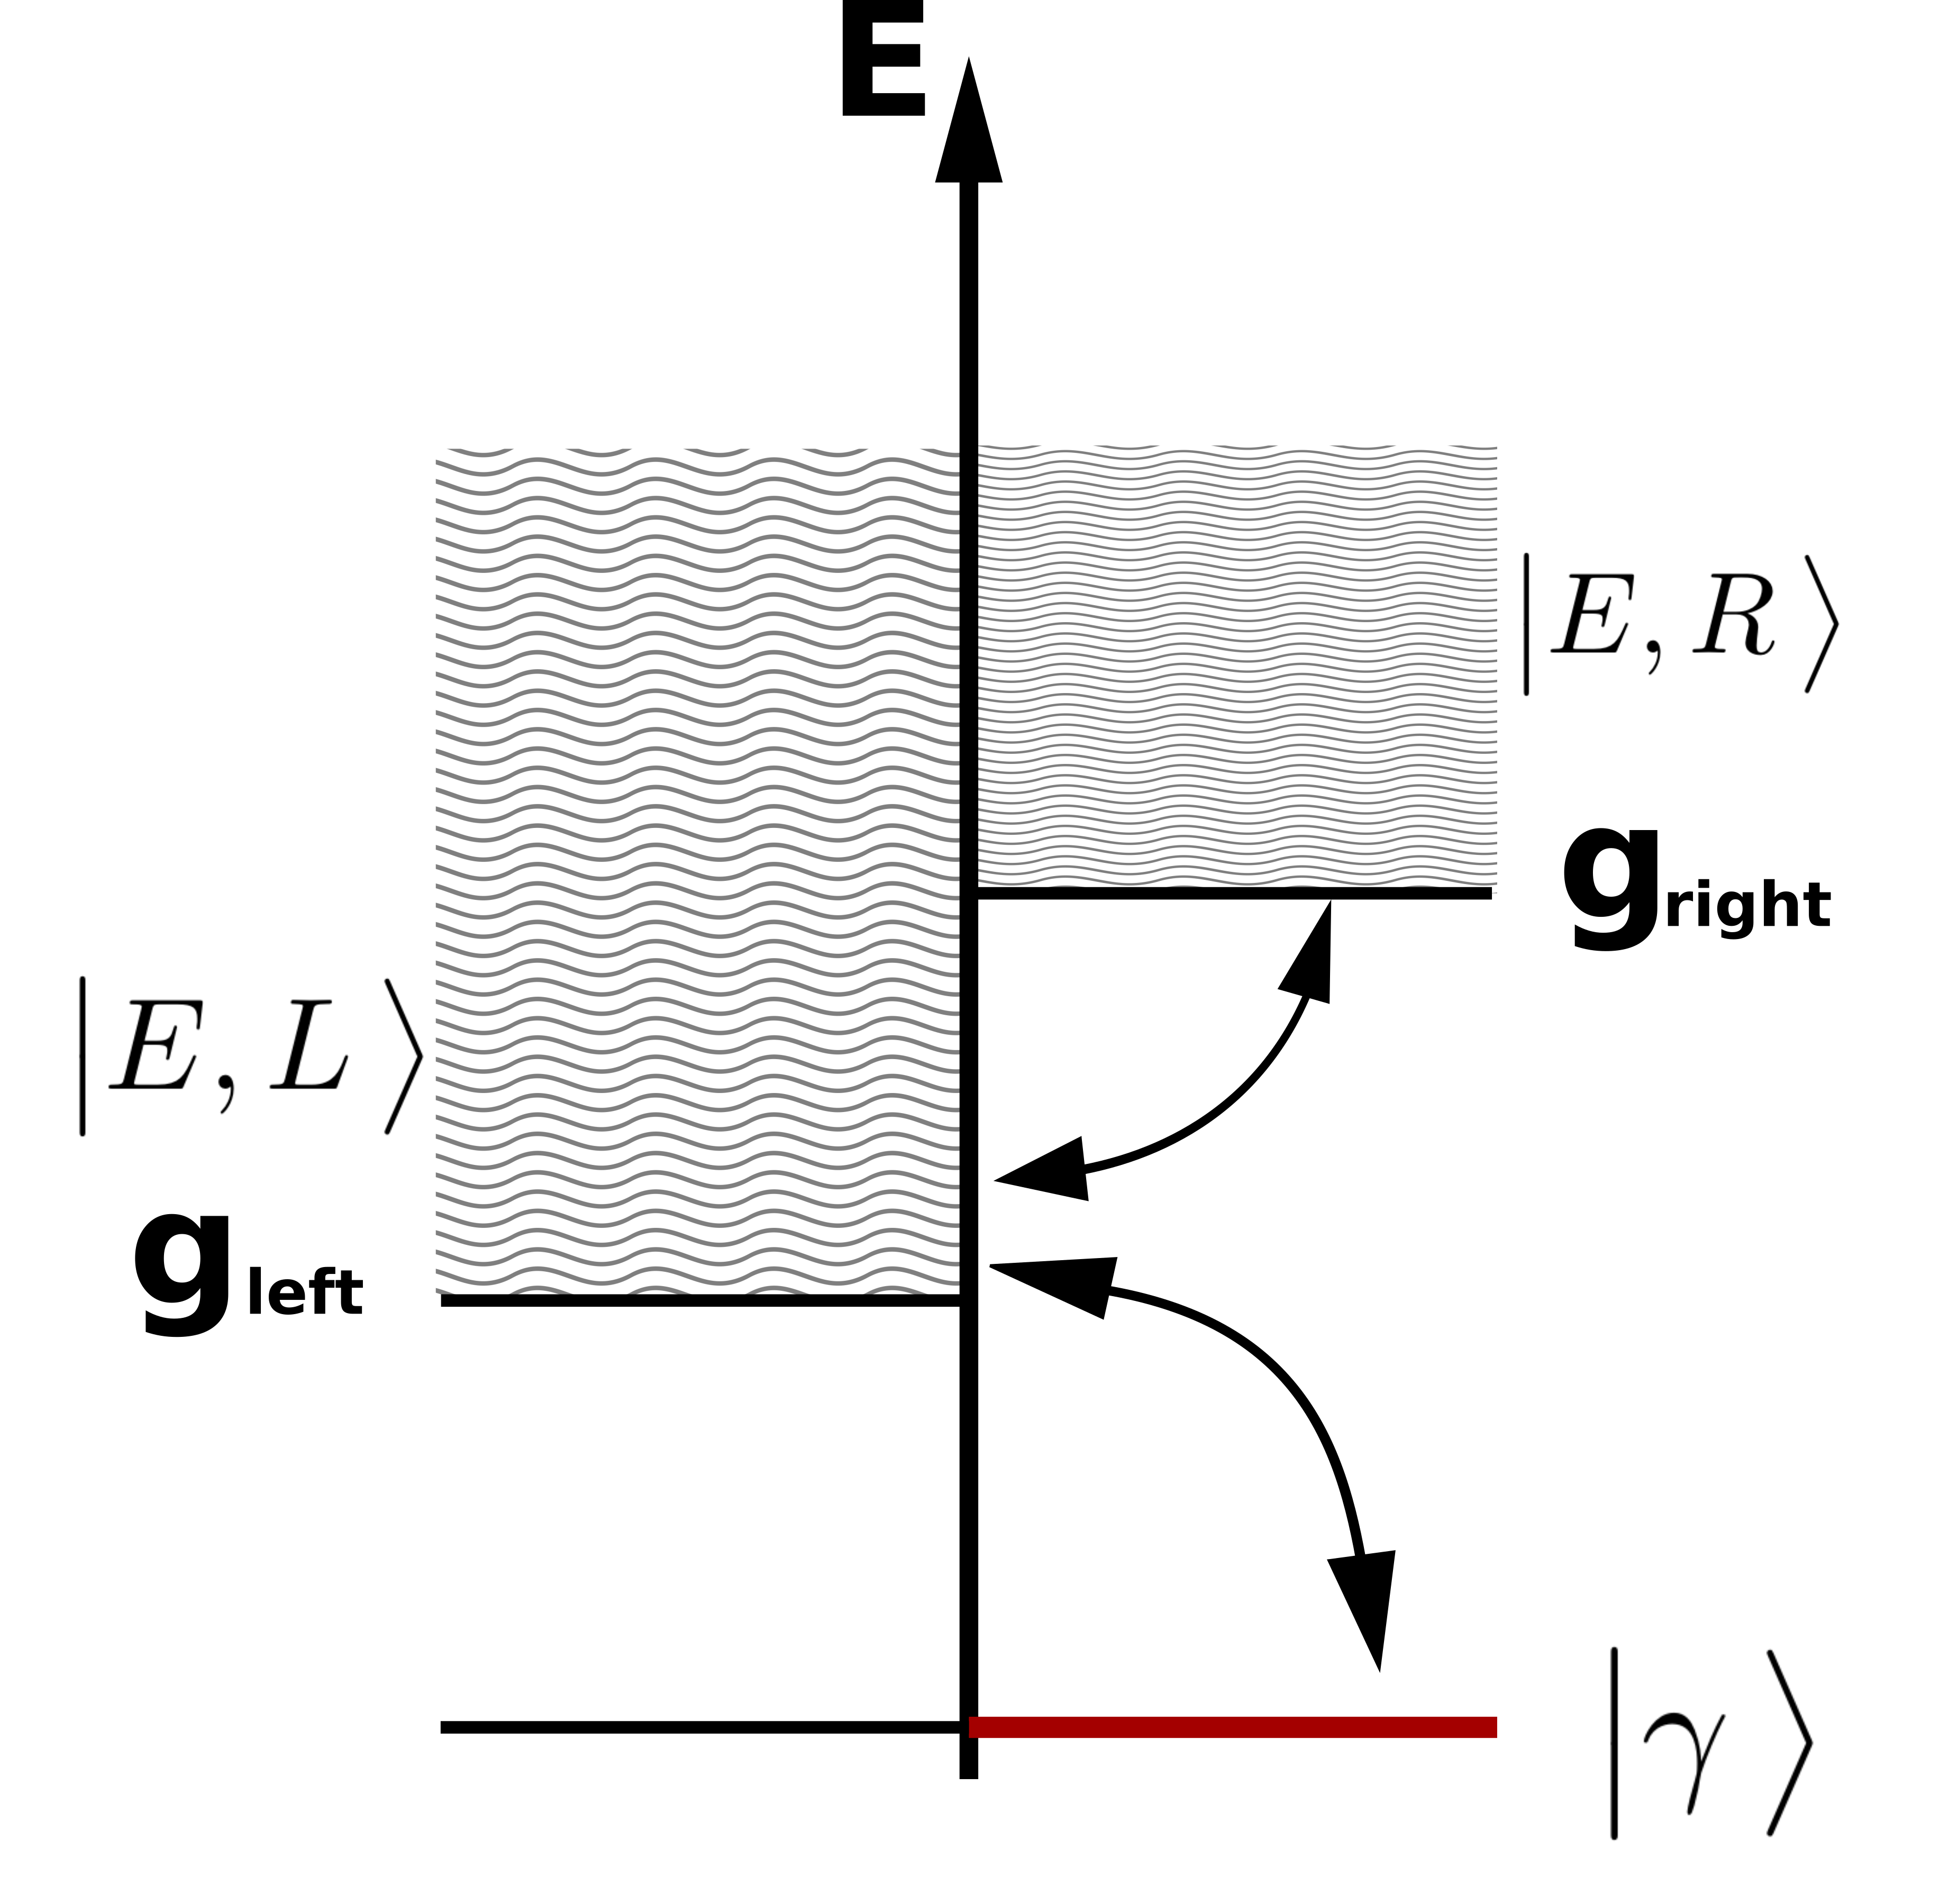
\includegraphics[width=0.65\linewidth]{images/tunneling}
	\caption{Ionization processes in terms of tunnel Hamiltonian}
	\label{fig:tunneling}
\end{figure}

The approach to multiphoton ionization is described in appendix \ref{app:multiphoton ionization}. The rate is given by the formula   (\ref{ionization_key}). To use this formula, we decompose the  perturbation in Fourier series. From  (\ref{tunnel_matrix_elements_maj-cont}) one finds, that $ V=H_T\propto\cos\frac{\varphi\br{\tau}}{2} $ with $ \varphi\br{\tau}=\varphi_{0}+\alpha\cos\omega \tau $. Using $ \alpha\ll1 $, we write:
\begin{multline}
	e^{\frac{i\varphi\br{\tau}}{2}}+e^{-\frac{i\varphi\br{\tau}}{2}}\simeq e^{i\frac{\varphi_{0}}{2}}\sum_{n}\frac{(i\alpha)^{n}}{2^{n}n!}(e^{in\omega \tau}+e^{-in\omega \tau})+c.c=
	\\
	=\sum_{n}\frac{\alpha{}^{n}}{2^{2n-1}n!}(e^{in\omega \tau}+e^{-in\omega \tau})\cos\left(\frac{\varphi_{0}}{2}+n\frac{\pi}{2}\right)
\end{multline}
so:
\begin{gather}
	h_{T}=
	\sum_n
	h_{T,n}
	\br{
	e^{in\omega }
	+
	e^{-in\omega }
	}
	\qquad
	h_{T,n}
	\approx
	\sum_{n}	
	\frac
	{\alpha^{n}}
	{2^{2n-1}n!}
	\cos\left(\frac{\varphi_{0}}{2}+n\frac{\pi}{2}\right)
	\tilde{h}_{T}
\end{gather}
Here the focus is on the case where the topological gap is much larger than the trivial one: $ \abs{g_L}\ll g_R $. In this case, the right continuum has high energies and does not participate in the ionization process. Indeed,
\begin{gather}
	h_T G_{\epsilon} h_T
	=
	\frac{h_T|\gamma\rangle\langle\gamma|h_T}{\epsilon}
	+
	\intop_{|E|>g_{R}}
	\frac{h_T|E,R_0\rangle\langle E,R_0|h_T}{\epsilon-E}\frac{dE}{N_{R}(E)}
\end{gather}
So, when $ g_{R}\gg\epsilon\sim \abs{g_L} $, the second term is small and can be neglected. Then, the product $ \dots h_TG\br{E}h_TG\br{E}h_T\dots $ factorizes into individual factors of the form $ J_{nm}\equiv\langle\gamma|h_{T,n}G\br{E}h_{T,m}|\gamma\rangle $.

\subsection{Factorizing $ w_\mathcal{E} $}
As each entry in the sum within $ w_{\mathcal{E}} $ has the form $ \dots h_TG\br{E}h_TG\br{E}h_T\dots $.  For ionization rate we have:
\begin{gather}
	\sqrt{\mathcal{I}}\propto
	\sum_N \sum_{\{n_i\}_M^N}\prod_{i=1}^{N}J_{n_in_{i+1}}
\end{gather}
Here $ N $ has the meaning of total number of absorbed photons, $ M $ is the closest to $ \frac{\abs{g_L}}{\omega }$ integer, and the second sum is taken over all sets $ \{n_i\}_M^N $ of $ N $ items and $ \sum_i^N n_{i=1} = M$.

 The $ n $,$ m $-dependence factors out:
\begin{gather}
J_{nm}
=
	\frac{\alpha^{n+m}}
	{2^{2\br{n+m}-2}n!m!}
	\cos\left(\frac{\varphi_{0}}{2}+n\frac{\pi}{2}\right)
	\cos\left(\frac{\varphi_{0}}{2}+m\frac{\pi}{2}\right)
	J_0\br{E}
\end{gather}
\begin{gather}
	J_{0}(E)
	=
	\langle\gamma|\tilde{h}_{T}G(E)\tilde{h}_{T}|\gamma\rangle
	\equiv
	\intop_{cont.}\frac{|\langle\gamma|\tilde{h}_{T}|\epsilon\rangle|^{2}}{E-\epsilon}\frac{d\epsilon}{N_L(\epsilon)}
\end{gather}

On each ionization step  the particle can move to the state with energy $ E $ or $ -E $, so:
\begin{gather}
	J_{0}(E)
	=
	2E\intop_{|g_{L}|}^{\infty}\frac{|\langle\gamma|\tilde{h}_{T}|\epsilon\rangle|^{2}}{E^{2}-\epsilon^{2}}\frac{d\epsilon}{N_L(\epsilon)}
\end{gather}
recalling (\ref{tunnel_matrix_elements_maj-cont}), we obtain:
\begin{gather}
		J_{0}(E)
		=
		ET\frac{\left[-1+\sqrt{1-\lambda^{2}}\right]}{\lambda^{2}}
\end{gather}
where $ \lambda = \frac{E}{\abs{g_L}} $, $ T=\frac{g_R\br{\zeta^2t}^2}{\abs{g_L}} $.

Thus, the elementary block  in our product for small enough $ n $ becomes:
\begin{gather}
	\frac{J_{nm}}{E+n\omega}
	\approx
	\frac{J_{nm}}{E}
	=
	\br{\frac{\alpha}{4}}^{n+m}
	B_n B_m^* T
	\frac{-1+\sqrt{1-\lambda^2}}{\lambda^2}
\end{gather}
where
\begin{gather}
	B_n=
	\frac{2}{n!}\cos\br{\frac{\phi_0}{2}+\frac{\pi n}{2}}
\end{gather}

The prefactor $  \br{\alpha/4}^{n+m} $ yields $ (\alpha/4)^{\mathcal{E}/\omega} $ for any trajectory and therefore do not affect summation and optimization. Thus one has $ B_{n}B_{m}T\frac{-1+\sqrt{1-\lambda^{2}}}{\lambda^{2}} $ to optimize.

Now consider a slice of the ionization process, i.e. a part of the full ionization product, which runs from energy $ E $ to $ E+\Delta E $ where $ \Delta E=M\omega $ with a large M. One can assume that within that process, a large number 2N of photons is absorbed, but energy does not change significantly, $ \Delta E\ll E $, so that $ \lambda $ can be considered a constant within that process. Denoting:
\begin{gather}
	T_{\lambda}=-4T\frac{\left[-1+\sqrt{1-\lambda^{2}}\right]}{\lambda^{2}}
\end{gather}
Then, one finds, that the ionization rate is $ \mathcal{I}\propto\mathcal{J}^2 $ where:
\begin{gather}
\label{ionization_super_formula}
\mathcal{J}
\equiv
\sum_N
\sum_{\{n\}_{N}^{M}}\prod_{i=1}^{N}\frac{J_{n_{i}n_{i+1}}}{E}
=
\left(\frac{\alpha}{4}\right)^{M}
\sum_N
\sum_{\{n\}_{2N}^{M}}(-T_{\lambda})^{\frac{N}{2}}\prod_{i=1}^{N}\frac{\cos(\frac{\varphi_{0}}{2}+\frac{\pi n_{2i}}{2})}{n_{i}!}
\end{gather}
So to obtain the ionization rate up to a prexponential constant, one should compute $ \mathcal{J} $.

\subsection{Using multinomial formula}
The first step to deal with (\ref{ionization_super_formula}) is to rewrite the product of cosines using multinomial formula:
\begin{gather}
	\frac{d^n}{dx^n}
	\prod_i f_i\br{x}
	=
	\sum_{\sum_i k_i=n}
	\begin{pmatrix}
	n
	\\
	k_1,k_2,\dots,k_n
	\end{pmatrix}
	\prod_i
	f_i^{(k_i)}
\end{gather}
For the cosine product it can be applied in a following way:
\begin{gather}
	\sum_{\{n\}_{N}^{M}}\prod_{i=1}^{N}\frac{\cos(\chi+\frac{\pi n_{i}}{2})}{n_{i}!}=\sum_{\{n\}_{N}^{M}}\prod_{i=1}^{N}\frac{D_{\chi}^{n_{i}}}{n_{i}!}\cos\chi=\frac{1}{M!}D_{\chi}^{M}\cos^{N}\chi
\end{gather}
where $ \chi=\frac{\varphi_0 }{2}$. Then some algebra should be used:
\begin{multline}
\label{after_multinomial}
	\frac{1}{M!}D_{\chi}^{M}\cos^{N}\chi=
	\frac{1}{2^{N}M!}D_{\chi}^{M}\sum_{k=0}^{N}C_{k}^{N}e^{i\chi(N-2k)}
	=
	\frac{e^{i\chi N+iM\pi/2}}{2^{N}M!}\sum_{k=0}^{N}C_{k}^{N}(N-2k)^{M}e^{-2ki\chi}
\end{multline}
Now, in the sum, the ratio of consecutive summands is $ \frac{a_{k+1}}{a_{k}}=\frac{C_{k+1}^{N}}{C_{k}^{N}}\left(\frac{N-2k-2}{N-2k}\right)^{M} $. For $ k<N/2 $ both factors here are decreasing, so the largest ratio is $ \frac{a_{1}}{a_{0}}=N(\frac{N-2}{N})^{M}\simeq Ne^{-2M/N} $. The most important terms in this sum define in wich regime the system is and what the ionization rate would be. 

The expression (\ref{ionization_super_formula}) can be rewritten with the help of the Poisson summation formula:

\begin{gather}
	\mathcal{J}
	=
	\br{\frac{\alpha}{4}}^M
	\sum_N
	\mathcal{J}_{N}	
\end{gather}
One can anticipate that the typical (i.e. most important) value of $ N $ is given by $ N_{*}=\frac{2M}{n_{*}} $ with $ n_{*}=\log\frac{1}{T_{\lambda}} $. It can be shown from considering the action $ s=\log\frac{1}{T_\lambda}-\frac{2}{2M} $ which appears in this sum. Taking $ N=N_{*} $ one can rewrite the condition $ \abs{\frac{a_{1}}{a_{0}}}\ll1 $ as $ \frac{2M}{n_{*}}\ll e^{n_{*}} $. This condition separates two regimes of the system --- pure Andreev regime, when only the first and the last terms in the sum are relevant, and the Andreev+Normal regime, when other terms should be taken into account.

\subsection{Pure Andreev regime}

When $ \frac{2M}{n_{*}}\ll e^{n_{*}} $ the sum (\ref{after_multinomial}) can be rewritten as:
\begin{gather}
	\mathcal{J}\approx\left(\frac{\alpha}{4}\right)^{M}\sum_{N}(-T_{\lambda})^{N/2}\frac{N^{M}}{M!2^{N}}\times2\cos\left(\chi N+\frac{M\pi}{2}\right)
\end{gather}
The preexponent is not the object of interest, while the fixed parity of N should be taken into account (it is fixed since the continuum state is available only on the left side of the junction). Replace $ N=2K $ and obtain:
\begin{multline}
	I_{M}=\left(\frac{\alpha}{4}\right)^{M}\sum_{K=1}^{\infty}(-T_{\lambda})^{K}\frac{(2K)^{M}}{M!2^{2K}}\times2\cos\left(\phi_{0}K+\frac{M\pi}{2}\right)=
	\\
	=\frac{2}{M!}\left(\frac{\alpha}{4}\right)^{M}\Re\left[i^{M}\sum_{K}(-T_{\lambda})^{K}\frac{(2K)^{M}}{2^{2K}}e^{i\phi_{0}K}\right]=\\=\frac{2^{M+1}}{M!}\left(\frac{\alpha}{4}\right)^{M}\Re\left[i^{M}\li_{-M}\left(\frac{T_{\lambda}}{4}e^{i(\phi_{0}+\pi)}\right)\right]
\end{multline}
%****************************************************************************
The polylogarithmic function can be rewritten in the following useful way
\[
\li_{s}(e^{\mu})=\Gamma(1-s)\sum_{r\in\mathbb{Z}}(2r\pi i-\mu)^{s-1}
\]

Substituting, we get
\[
\li_{-M}\left(\frac{T_{\lambda}}{4}e^{i(\phi_{0}+\pi)}\right)=\Gamma(1+M)\sum_{r\in\mathbb{Z}}\left(i[2r\pi-\pi-\phi_{0}]+\ln\frac{4}{T_{\lambda}}\right)^{-M-1}
\]

Denoting $\ln\frac{4}{T_{\lambda}}=n_{\lambda}$ we have the ratio
of consecutive terms in the sum (assuming they are not too far from
the largest term):
\[
\left|\frac{a_{r+1}}{a_{r}}\right|\sim\left(\frac{n_{\lambda}^{2}+(\gamma_{r}+2\pi)^{2}}{n_{\lambda}^{2}+\gamma_{r}^{2}}\right)^{-1-M}\sim\left(1+\frac{2\pi(2\pi+2\gamma_{r})}{n_{\lambda}^{2}+\gamma_{r}^{2}}\right)^{-M}\sim\exp\left[\frac{4\pi M(\pi+\gamma_{r})}{n_{\lambda}^{2}}\right]
\]

where $\gamma_{r}=i(2r\pi-\pi-\phi_{0})$. There are two values of
$r$ for which $|\pi+\gamma_{r}|$ is smallest, for the rest it is
not smaller than $2\pi$ so that the rest of the terms are smaller
by at least 
\[
\exp\left[-\frac{8\pi^{2}M}{n_{\lambda}^{2}}\right]
\]

\textbf{Subcase}
\[
\exp\left[\frac{8\pi^{2}M}{n_{\lambda}^{2}}\right]\gg1
\]
in which case the sum over $r$ is dominated by the two largest terms
(typically by just one term except for the case when $\phi_{0}$ is
close to zero). We dictate $-\pi<\phi_{0}<\pi$ so that the two dominating
terms correspond to $r=0,1$. We have in that limit

\[
\li_{-M}\left(\frac{T_{\lambda}}{4}e^{i(\phi_{0}+\pi)}\right)\simeq M!\left(\frac{1}{(n_{\lambda}+i(\pi-\phi_{0}))^{M+1}}+\frac{1}{(n_{\lambda}+i(-\pi-\phi_{0}))^{M+1}}\right)
\]

and thus 
\[
I_{M}=2\left(\frac{\alpha}{2}\right)^{M}\Re\left[i^{M}\left(\frac{1}{(n_{\lambda}+i(\pi-\phi_{0}))^{M+1}}+\frac{1}{(n_{\lambda}+i(-\pi-\phi_{0}))^{M+1}}\right)\right]
\]

We have 
\[
[n_{\lambda}+i(\pi-\phi_{0})]^{M+1}=\left[n_{\lambda}^{2}+(\pi-\phi_{0})^{2}\right]^{\frac{M+1}{2}}e^{i(M+1)\arctan\frac{\pi-\phi_{0}}{n_{\lambda}}}
\]
and 
\begin{align*}
I_{M} & =2\left(\frac{\alpha}{2}\right)^{M}\Re\left[\frac{e^{\frac{iM\pi}{2}-i(M+1)\arctan\frac{\pi-\varphi_{0}}{n_{\lambda}}}}{\left[n_{\lambda}^{2}+(\pi-\phi_{0})^{2}\right]^{\frac{M+1}{2}}}+\frac{e^{\frac{iM\pi}{2}+i(M+1)\arctan\frac{\pi+\varphi_{0}}{n_{\lambda}}}}{\left[n_{\lambda}^{2}+(\pi+\phi_{0})^{2}\right]^{\frac{M+1}{2}}}\right]=\\
& =2\left(\frac{\alpha}{2}\right)^{M}\left[\frac{\cos\left(\frac{M\pi}{2}-(M+1)\arctan\frac{\pi-\varphi_{0}}{n_{\lambda}}\right)}{\left[n_{\lambda}^{2}+(\pi-\phi_{0})^{2}\right]^{\frac{M+1}{2}}}+\frac{\cos\left(\frac{M\pi}{2}+(M+1)\arctan\frac{\pi+\varphi_{0}}{n_{\lambda}}\right)}{\left[n_{\lambda}^{2}+(\pi+\phi_{0})^{2}\right]^{\frac{M+1}{2}}}\right]
\end{align*}

This contains some complicated oscillations but within exponential
accuracy we may write
\[
I_{M}\sim\exp M\left[\ln\frac{\alpha}{2}-\frac{1}{2}\ln(n_{\lambda}^{2}+(\pi-|\varphi_{0}|)^{2})\right]
\]

This is almost the final formula for the ionization amplitude. To
finalize it, we have to replace the action at fixed $n_{\lambda}$
by an integration over $\lambda$ to account for the slowly changing
energy of the quasiparticle. However,it is unclear, what is required
of $M,n_{*}$ to allow such a procedure. The procedure assumes that
we can roughly write $I_{M}=\prod_{j}I_{M_{j}}(\lambda_{j})$ where
the full process is split into layers counted by $j$ where within
each layer energy if roughly the same and $\sum M_{j}=M$, but $M_{j}$
is relatively large (so that $N_{j}$ remains large). Hypothetically,
if our principal conditions are met (the ones that limit the sum to
highest harmonics and allow the use of asymptotics for $\li$) then
we can split $M$ into layers which individually obey the same limits.
Therefore, in the mathematical limit the procedure seems correct,
but it is hard to tell, what accuracy it has. We have
\begin{align*}
s_{\lambda} & =\intop_{0}^{1}\ln(n_{\lambda}^{2}+(\pi-|\varphi_{0}|)^{2})d\lambda=\intop_{0}^{1}\ln(\ln(\frac{4}{T_{\lambda}})^{2}+(\pi-|\varphi_{0}|)^{2})d\lambda\\
& =\intop_{0}^{1}\ln\left(\left[\ln\frac{\lambda^{2}}{T_{0}(1-\sqrt{1-\lambda^{2}})}\right]^{2}+(\pi-|\varphi_{0}|)^{2}\right)d\lambda
\end{align*}

Calculation of the $\lambda$-integral:

\[
\intop_{0}^{1}\ln(n_{\lambda}^{2}+(\pi-|\varphi_{0}|)^{2})d\lambda=\intop_{0}^{1}\left(2\ln n_{\lambda}+\frac{(\pi-|\varphi_{0}|)^{2}}{n_{\lambda}^{2}}\right)d\lambda
\]

Separately we find:
\[
\intop_{0}^{1}\ln n_{\lambda}d\lambda=\ln\frac{1}{T}+\intop_{0}^{1}\ln\frac{\lambda^{2}}{1-\sqrt{1-\lambda^{2}}}d\lambda=\ln\frac{1}{T}+\frac{\pi}{2}-1.
\]

For the second integral we have
\[
\intop_{0}^{1}\frac{1}{n_{\lambda}^{2}}d\lambda=\intop_{0}^{1}\frac{1}{\left[\ln\frac{1}{T}+\ln\frac{\lambda^{2}}{1-\sqrt{1-\lambda^{2}}}\right]^{2}}d\lambda=\frac{1}{(\ln\frac{1}{T})^{2}}+O\left(\frac{1}{(\ln\frac{1}{T})^{3}}\right)
\]

Thus, we get 
\[
s_{\lambda}=2\ln\frac{1}{T}+\pi-2+\frac{(\pi-|\varphi_{0}|)^{2}}{(\ln\frac{1}{T})^{2}}+O\left(\frac{1}{(\ln\frac{1}{T})^{3}}\right)
\]

and the final result in this limit (only pure MAR (multiple Andreev
reflections)) is:
\[
P=\exp\left[-\frac{g_{L}}{\omega}\left(2\ln\frac{2}{\alpha}+2\ln\ln\frac{1}{T}+\pi-2+\frac{(\pi-|\varphi_{0}|)^{2}}{(\ln\frac{1}{T})^{2}}+O\left(\frac{1}{(\ln\frac{1}{T})^{3}}\right)\right)\right]
\]

\[
(\ln\frac{1}{T})^{2}\ll\frac{g_{L}}{\omega}\ll(\ln\frac{1}{T})^{2}e^{1/T}
\]

and in the second regime,

\[
P=\exp\left[-\frac{g_{L}}{\omega}\left(2\ln\frac{2}{\alpha}+2\ln\ln\frac{1}{T}+\pi-2+o(1)\right)\right]
\]

\[
(\ln\frac{1}{T})^{2}\ll\frac{g_{L}}{\omega}
\]
This includes the previous answer. The $o(1)$ is to be determined.

Finally, in the case where $n_{*}\ll M\ll n_{*}^{2}$ I do Poisson
to calculate $\li$ and find that it behaves strangely: I get $e^{-M\ln n_{\lambda}-\frac{1}{2}{\frac{M}{n_{\lambda}}}^{2}n_{\lambda}^{2}/M+corr.}$
where ${M/n_{\lambda}}$ denotes the fractional part of the number
(from $-1/2$ to $1/2$). The number within changes quickly with $\lambda$
and therefore $^{2}\rightarrow\langle{}^{2}\rangle=1/12$. Then, we
get
\begin{align}
P & =\exp\left[-\frac{g_{L}}{\omega}\left(2\ln\frac{2}{\alpha}+2\ln\ln\frac{1}{T}+\pi-2\right)+\frac{1}{12}\frac{(\ln\frac{1}{T})^{2}}{g_{L}/\omega}+o\left(\frac{(\ln\frac{1}{T})^{2}}{g_{L}/\omega}\right)\right]
\end{align}
\begin{gather}
	\qquad(\ln\frac{1}{T})\ll\frac{g_{L}}{\omega}<(\ln\frac{1}{T})^{2}\
\end{gather}

\subsubsection{Pure Andreev regime regime: intermediate case: fixed photon number}

Above we considered $M\gg n_{*}$ which lead to a simple asymptotic
of the function $\li_{-M}(e^{-n_{*}+i(\phi_{0}+\pi)})$. There is
also the intermediate case where $n_{*}\ll M\ll n_{*}^{2}$. In this
case the dominating term(s) have large index $K$, but the gaussian
envelope is very narrow, with a width $\ll1$ which means that the
full series is dominated by a single term (this is in full agreement
with the fact that the second form of $\li$ is now wide, i.e. converges
over a large number of $r$-terms). It is easy to show that the optimal
term has the integer index $K_{0}$ closest to the real saddle-point
$K_{*}=M/n_{*}$. We write
\[
K_{*}=K_{0}+\xi,\qquad\mbox{with\ensuremath{\qquad\xi\in(-\frac{1}{2},\frac{1}{2})}}
\]

Then, omitting the complex phase, we write
\begin{multline*}
\li_{-M}(e^{-n_{*}+i(\phi_{0}+\pi)})\approx a_{K_{0}}\propto e^{-n_{*}(K_{*}-\xi)+M\ln(K_{0}-\xi)}=\\
=e^{-M+n_{*}\xi+M\ln\frac{M}{n_{*}}+M\ln(1-\frac{\xi n_{*}}{M})}=e^{-M+M\ln\frac{M}{n_{*}}-\frac{\xi^{2}n_{*}^{2}}{2M}+O\left(\frac{n_{*}^{3}}{M^{2}}\right)}\\
\end{multline*}

Substituting this result for the $\li$ function we obtain in this
regime (to exponential accuracy)
\[
I\sim\frac{1}{M!}(\frac{\alpha}{2})^{M}e^{-M+M\ln\frac{M}{n_{*}}-\frac{\xi^{2}n_{*}^{2}}{2M}+O\left(\frac{n_{*}^{3}}{M^{2}}\right)}=e^{-M\ln\frac{2}{\alpha}-M\ln n_{*}-\frac{\xi^{2}n_{*}^{2}}{2M}++O\left(\frac{\xi^{3}n_{*}^{3}}{M^{2}}\right)}
\]

and for the probability we write:
\[
P_{2}=\exp\left[-M\left(2\ln\frac{2}{\alpha}+2\ln n_{*}\right)-\left\{ \frac{M}{n_{*}}\right\} ^{2}\frac{n_{*}^{2}}{M}+O\left(\frac{n_{*}^{3}}{M^{2}}\right)\right],\qquad n_{*}\ll M\ll n_{*}^{2}
\]

\subsection{Andreev+Normal regime}

For completenness, let us also consider the case $M/N\ll\log N$.
In this case the sum over $k$ is not defined by the two edge terms.
We write:
\[
\sum_{k=0}^{N}C_{k}^{N}(N-2k)^{M}e^{-2ki\chi}=\sum_{k=0}^{N}e^{-S_{0}(k)-2ki\chi}
\]

where the action $S_{0}$ is 
\begin{multline*}
S_{0}=-\ln C_{k}^{N}-M\ln(N-2k)=-N\ln N+k\ln k+(N-k)\ln(N-k)-\\
-M\ln(N-2k)-\frac{1}{2}\ln\frac{N}{2\pi(N-k)k}+\dots
\end{multline*}

The stationary point of that action obeys $\partial S_{0}/\partial k=0$:
\[
\ln k-\ln(N-k)+\frac{2M}{N-2k}+\frac{1}{2k}-\frac{1}{2(N-k)}=0
\]

As expected, $k\to N-k$ changes the sign of this. We seek for the
stationary point with $k<N/2$. We have the transcendent equation
(terms $\sim1/k,1/N$ are neglected)
\[
\ln(\frac{N}{k}-1)=\frac{2M/N}{1-2k/N}
\]

This is generally unsolvable, but if we assume that $M/N\gg1$ then
we get $k/N\ll1$ and the asymptotics is
\begin{align*}
-\ln\frac{k}{N} & =2\frac{M}{N}\\
\\
k_{0} & =Ne^{-2M/N}
\end{align*}

We remind that this happens in the regimes $1\ll M/N\ll\ln N$. At
the same time, to have $k\gg1$ produces the additional constraint
$M/N\ll\frac{1}{2}\ln N$. At this saddle point, $k=k_{0}$, we have
\[
\frac{\partial^{2}S_{0}}{\partial k^{2}}\approx\frac{1}{k}+\frac{1}{N-k}+\frac{4M}{(N-2k)^{2}}\approx\frac{1}{k_{0}}+\frac{4M}{N^{2}}=\frac{1}{N}\left(e^{2M/N}+\frac{4M}{N}\right)\approx\frac{1}{k_{0}}
\]

where we made use of $M/N\gg1$. The action itself if 
\begin{multline*}
S_{0}=-N\ln N+k_{0}\ln k_{0}+(N-k_{0})\ln(N-k_{0})-M\ln(N-2k_{0})-\frac{1}{2}\ln\frac{N}{2\pi(N-k_{0})k_{0}}\\
\approx-N\ln N+k_{0}\ln k_{0}+(N-k_{0})\left[\ln N+\ln(1-\frac{k_{0}}{N})\right]-\\
-M\left[\ln N+\ln(1-\frac{2k_{0}}{N})\right]-\frac{1}{2}\ln\frac{1}{2\pi k_{0}}+\frac{1}{2}\ln(1-\frac{k_{0}}{N})
\end{multline*}

If we are interested in the exponent and preexponent, we can only
omit terms of the order $o(1)$ in $S_{0}$, for example the very
last term in the above. We get
\[
S_{0}\approx-(M+k_{0})\ln N+(k_{0}+\frac{1}{2})\ln k_{0}+(N-k_{0})\ln(1-\frac{k_{0}}{N})-M\ln(1-\frac{2k_{0}}{N})-\frac{1}{2}\ln\frac{1}{2\pi}
\]

However, since our solution for $k_{0}$ is itself approximate, we
should restrict ourselves to exponential accuracy here and keep only
major terms, linear in $M$
\begin{align*}
S_{0} & =-M\ln N+O(k_{0}\frac{M}{N},k_{0}\ln N,k_{0},k_{0}\ln k_{0})\\
& =-M\ln N+O(k_{0}\ln N)
\end{align*}

We now integrate using the Poisson formula:
\begin{align*}
\sum_{k=0}^{N/2}e^{-S_{0}(k)-2ki\chi} & =\sum_{p\in\mathbb{Z}}e^{-S_{0}(k_{0})-2k_{0}i(\chi-\pi p)}\int dke^{-\frac{1}{2k_{0}}(k-k_{0})^{2}-2(k-k_{0})i(\chi-\pi p)}\\
& =\sum_{p\in\mathbb{Z}}e^{-S_{0}(k_{0})-2k_{0}i(\chi-\pi p)-2(\chi-\pi p)^{2}k_{0}}\sqrt{2\pi k_{0}}
\end{align*}

Assuming $\phi_{0}$ is not close to $\pm\pi$ the above is dominated
by the term with $p=0$ because $k_{0}\gg1$. If we are close to $\pi$
phase difference, there are two main terms, but, to an exponential
accuracy the answer is still the same (the only problem that could
possibly arise is alternating-sign sums that might appear later when
summing over $N$ and give incorrect results due to the approximation
we do now. Maybe this can be mended easily by restoring these terms
via replicating the result via $\phi_{0}\rightarrow\phi_{0}+2\pi p$).
In the above, we only integrated near the saddle-point with $k_{0}<N/2$,
there remains the symmetric saddle at $N-k_{0}$. This adds the complex
conjugate to the result (but first we must restore some prefactors):
\begin{multline*}
\frac{i^{M}e^{i\chi N}}{M!2^{N}}\sum_{k=0}^{N}C_{k}^{N}(N-2k)^{M}e^{-2ki\chi}=\\
\sqrt{2\pi k_{0}}\frac{e^{i\chi N+iM\pi/2}}{M!2^{N}}\sum_{p\in\mathbb{Z}}e^{-S_{0}(k_{0})-2k_{0}i(\chi-\pi p)-2(\chi-\pi p)^{2}k_{0}}+c.c.=\\
=2\frac{\sqrt{2\pi k_{0}}}{M!2^{N}}e^{-S_{0}}\sum_{p\in\mathbb{Z}}\exp\left[-2(\chi-\pi p)^{2}k_{0}\right]\cos\left[-2k_{0}(\chi-\pi p)+\chi N+\frac{M\pi}{2}\right]
\end{multline*}

The sum can be written in terms of the elliptic theta-function. But
thus is not particularly helpful. Instead, we risk omitting all terms
except the $p=0$ -terms. This preserves exponential accuracy, but
risks errors in further summation over $N$, since that summation
may be an alternating sign sum susceptible to minor corrections to
the terms. We get
\[
2\frac{\sqrt{2\pi k_{0}}}{M!2^{N}}e^{-S_{0}}\sum_{p\in\mathbb{Z}}\exp\left[-\chi^{2}k_{0}\right]\cos\left[\chi(N-2k_{0})+\frac{M\pi}{2}\right]
\]
The next step is to sum this over $N$. Remember that $k_{0}=Ne^{-2M/N}$
and $S_{0}=S_{0}(M,N,k_{0}(M,N))$. We now have
\[
\Re\frac{i^{M}}{M!}\left(\frac{\alpha}{4}\right)^{M}\sum_{N}\left(-\frac{T_{\lambda}}{4}\right)^{N/2}\sqrt{k_{0}}e^{-S_{0}-\chi^{2}k_{0}+i\chi(N-2k_{0})}
\]

where we omitted a few pre-exponential factors. We now replace $N=2K$
and rewrite:

\[
\frac{1}{M!}\left(\frac{\alpha}{4}\right)^{M}\Re i^{M}\sum_{N}\left(-\frac{T_{\lambda}}{4}\right)^{K}\sqrt{k_{0}}e^{-S_{0}-\frac{\phi_{0}^{2}k_{0}}{4}+i\phi_{0}(K-k_{0})},\qquad k_{0}=\frac{K}{2}e^{-M/K}
\]

We now again have to use the saddle appoximation when summing over
$K$. The total action, as a function of $K$ is
\[
S(K)=S_{0}+\frac{\phi_{0}^{2}k_{0}}{4}-i\phi_{0}(K-k_{0})-K\left(\frac{i\pi}{2}+\ln\frac{T_{\lambda}}{4}\right).
\]

We are again looking for the stationary point. At this point we calculate
$\partial S/\partial K$ to the main order. In particular, since we
expect $M\gg K$ we may neglect the $k_{0}$-terms that are seen explicitly:
we have
\begin{align*}
\frac{\partial S}{\partial K} & \simeq\frac{\partial S_{0}}{\partial K}+i\left(\phi_{0}+\frac{\pi}{2}+\ln\frac{T_{\lambda}}{4}\right)\\
& \simeq-\frac{M}{K}-\left(i\phi_{0}+i\frac{\pi}{2}+\ln\frac{T_{\lambda}}{4}\right)
\end{align*}

which immediately gives $K=M/n_{\lambda}$ where $n_{\lambda}=\ln(4/T_{\lambda})$.
This is the same size as before, which is a good sign! Thus, we mainly
have to calculate

The projected answer is:
\begin{align*}
I & =e^{-Ms}\\
s & =\ln\frac{2}{\alpha}+\intop_{0}^{1}\ln n_{\lambda}d\lambda+o(1)
\end{align*}

\textbf{Single-photon case.} Here we simply have one photon with $N=M$
which produces the $(\alpha/4)^{M}/M!$ factor and therefore, to exponential
accuracy we get

\[
P\sim T\exp\left[-M\left(2\ln\frac{4}{\alpha}-\ln M+1\right)\right]
\]


\section{Results}

Here we collect results for the ionization rate (i.e. probability
$P\propto I_{M}^{2}$) within exponential accuracy. There are for
parametric regimes (for now we forget about the adiabaticity condition
-- we will later discuss it). We have the notations $M=g_{L.}/\omega$
is the total number of energy quanta needed to ionize. We have $n_{*}=\ln\frac{1}{T}$
-- \textbf{twice} the optimal size of a photon (in quanta of $\omega$).
The amount of photons in a configuration is called $N$, its optimum
amount is $N_{*}=2M/n_{*}$. The results are as follows:

\subsubsection{Ionization rate}
\begin{enumerate}
	\item Single-photon case: $M<n_{*}$. In this case, the tunneling parameter
	$T$ is so small that it is best to use a single photon to minimize
	the $T^{N/2}$ factor in the amplitude $I_{NM}$. Then we have
	\begin{equation}
	P_{1}\sim T\exp\left[-M\left(2\ln\frac{4}{\alpha}-2\ln M+2\right)\right]
	\end{equation}
	\item Fixed number of photons case: $n_{*}\ll M\ll n_{*}^{2}$. In this
	case it is optimal to use multiple photons, more sepcifically exactly
	$N_{*}$ photons (rounded to the nearest integer, of course). Processes
	with different $N$ do not contribute (their contribution is negligible).
	We get
	\begin{equation}
	P_{N_{*}}\sim\exp\left[-M\left(2\ln\frac{2}{\alpha}+2\ln n_{*}+\pi-2+\left\{ \frac{M}{n_{*}}\right\} ^{2}\frac{n_{*}^{2}}{M^{2}}+O\left(\frac{n_{*}^{3}}{M^{3}}\right)\right)\right]
	\end{equation}
	\\
	Here $\{M/n_{*}\}\in(-0.5,0.5)$ stand for the fractional part of
	the argument (or rather distance to nearest integer). We see that
	integer effects are important in this regime.
	\item Fluctuating photon number case: $n_{*}^{2}\ll M$. Now, for combinatorial
	reasons, contributions from $N\neq N_{*}$ become important, and we
	get
	\begin{equation}
	P_{N_{*}+\delta N}\sim\exp\left[-M\left(2\ln\frac{2}{\alpha}+2\ln n_{*}+\pi-2+o(1)\right)\right]
	\end{equation}
	\\
	In this case $N$ fluctuates significantly ($\delta N=N-N_{*}$ is
	typically much larger than unity but much smaller than $N_{*}$. It
	can be found if needed). Thus, no integer effects remain.
	\item Sub-case of (3) where only Andreev reflection happens: $n_{*}^{2}\ll M\ll n_{*}e^{n_{*}}.$
	In thi case we take only left term in each cosine, or only right --
	this produces the largest contribution to ionization. {[}At higher
	$M$ some normal reflections start to happen (combinatorically they
	become important. Or, in other words, their phase space becomes large
	-- there are many such ``trajectories''). This case is very technically
	involved{]}. So, if only MAR (multiple Andreev reflection) happens,
	then we can furhter refine the expression for the ionization rate
	and get
	\begin{equation}
	P_{N_{*}+\delta N}^{(MAR)}\sim\exp\left[-M\left(2\ln\frac{2}{\alpha}+2\ln n_{*}+\pi-2+\frac{(\pi-|\varphi_{0}|)^{2}}{n_{*}^{2}}+O\left(\frac{1}{n_{*}^{3}}\right)\right)\right]
	\end{equation}
	\linebreak{}
	\textbf{Note on all cases and energy dependence}: the Green's function
	energy depends on the current energy (i.e. sum of energies of all
	previously absorbed photons). Therefore, $T$ becomes a function of
	$\lambda=E/g_{L}$. Note that this dependence is slow -- $T$ is
	rescaled by the very nice function $c(\lambda)=(1-\sqrt{1-\lambda^{2}})/\lambda^{2}\in(1/2,1)$.
	So that $n_{*}$ only changes by $-\ln c(0)=\ln2\simeq0.3$. This
	energy dependence is actually accounted for and is the origin of the
	$\pi-2$ terms in expressions for $P$.
\end{enumerate}
